\chapter{Glosario de términos}

Muchos de los términos utilizados en este documento, están referidos a
conceptos que mezclan terminología de Internet, psicología, y pedagogía.
Para evitar las ambigüedades en estos términos (que son de amplio uso en el
documento) se ha creado este anexo. Estos son:

\begin{description}
\item [Usuario:] Persona que tiene el potencial de utilizar el sistema, cosa
que no implica que lo use.
\item [Rol:] Definición del conjunto de funciones del sistema, disponibles para
los usuarios.
\item [Docente:] Tipo de rol definido en el sistema, y que tiene la intención
de representar a un profesor.
\item [Espacio virtual:] Lugar del sistema donde los usuarios pueden compartir
recursos.
\item [Materia:] Tipo de espacio virtual de tipo formal, que engloba una tópico
determinado y que puede contener uno o varios grupos.
\item [Grupo:] Tipo de espacio virtual de tipo formal, que es regida por un
docente y que define una forma de enseñanza independiente de otros espacios
virtuales.
\item [Recurso:] Pieza de información creada por los usuarios, que es
compartida a todos los usuarios de un espacio virtual determinado.
\item [Actividad:] Indicador del sistema que mide el numero de recursos creados
por un usuario.
\item [Participación:] Indicador del sistema que mide el numero de comentarios
creados por un usuario.
\item [Contactos:] Usuarios del sistema que poseen algún tipo de vinculo con 
otro usuario.
\item [Enlace débil:] Es el tipo de relación entre dos usuarios, en el que solo
uno de ellos reconoce al otro.
\item [Enlace fuerte:] Es el tipo de relación entre dos usuarios, en el que 
ambos se reconocen.
\item [Sociabilidad:] Indicador del sistema que mide el numero de enlaces, ya
sean fuertes o débiles, que posee un usuario.
\item [Popularidad:] Indicador del sistema que mide el grado de valoración de 
los usuarios hacia los recursos de un usuario.
\item [Audiencia:] Es el conjunto de usuarios que únicamente vieron el recurso,
sin realizar otra acción hacia este.
\item [Calificadores:] Es el conjunto de usuarios que mostraron un interés 
explicito hacia un recurso en particular.
\end{description}

Las relaciones existentes entre los elementos del sistema están resumidos en la
%Figura \ref{nomenclatura}.
%\begin{figure}
%\centering
%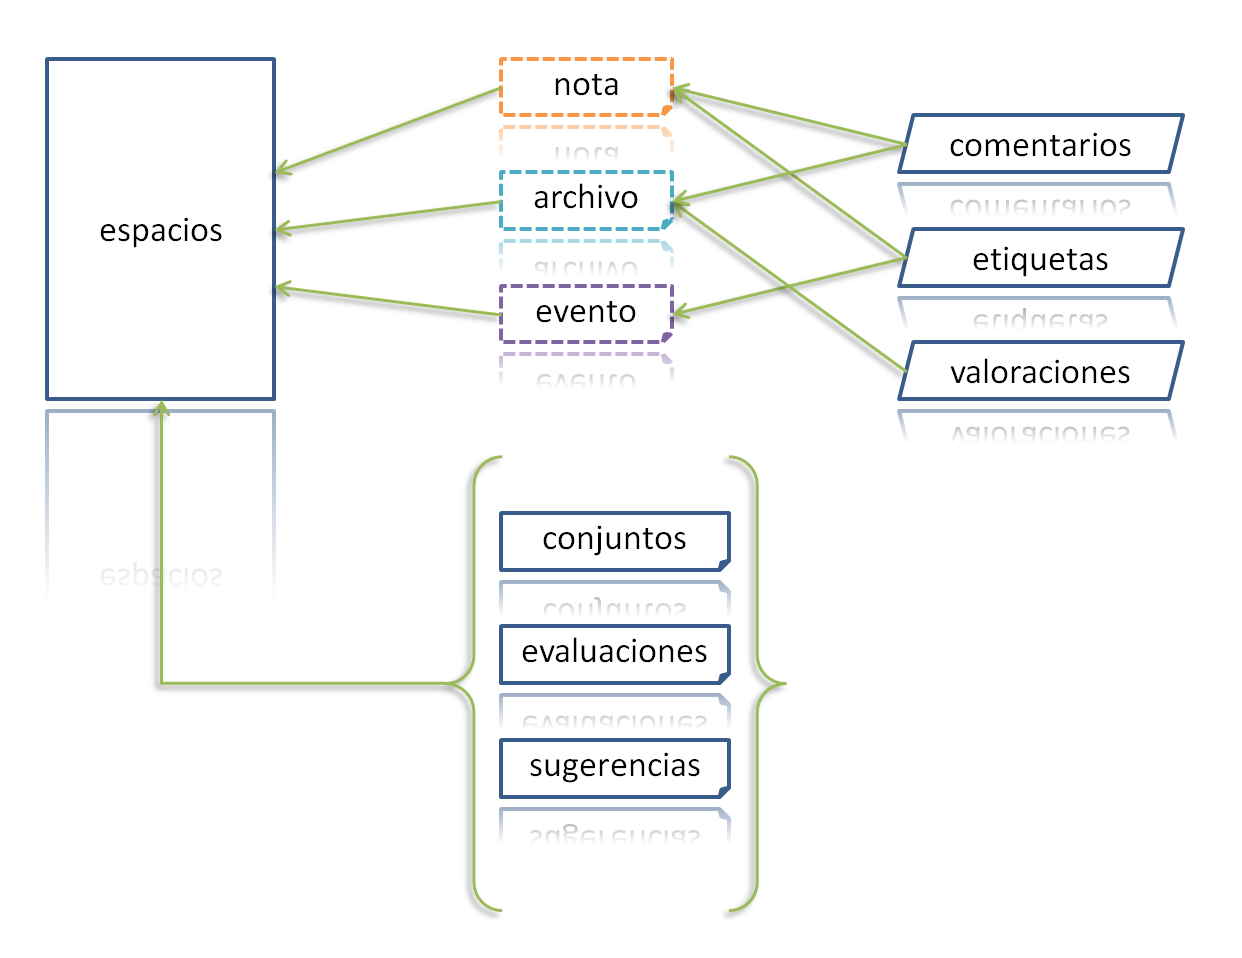
\includegraphics[scale=0.3]{graphics/nomenclatura.png}
%\caption {Relación entre los conceptos utilizados en el sistema}
%\label {nomenclatura}
%\end{figure}
